\subsection{Design du système}
    Le système se dècoupe essentiellement en 3 parties:
    \begin{itemize}
        \item[-] Coté utilisateur
        \item[-] Coté jeu
        \item[-] Coté Server   
    \end{itemize}
    \subsubsection{Coté utilisateur}
        % \makebox[\textwidth]{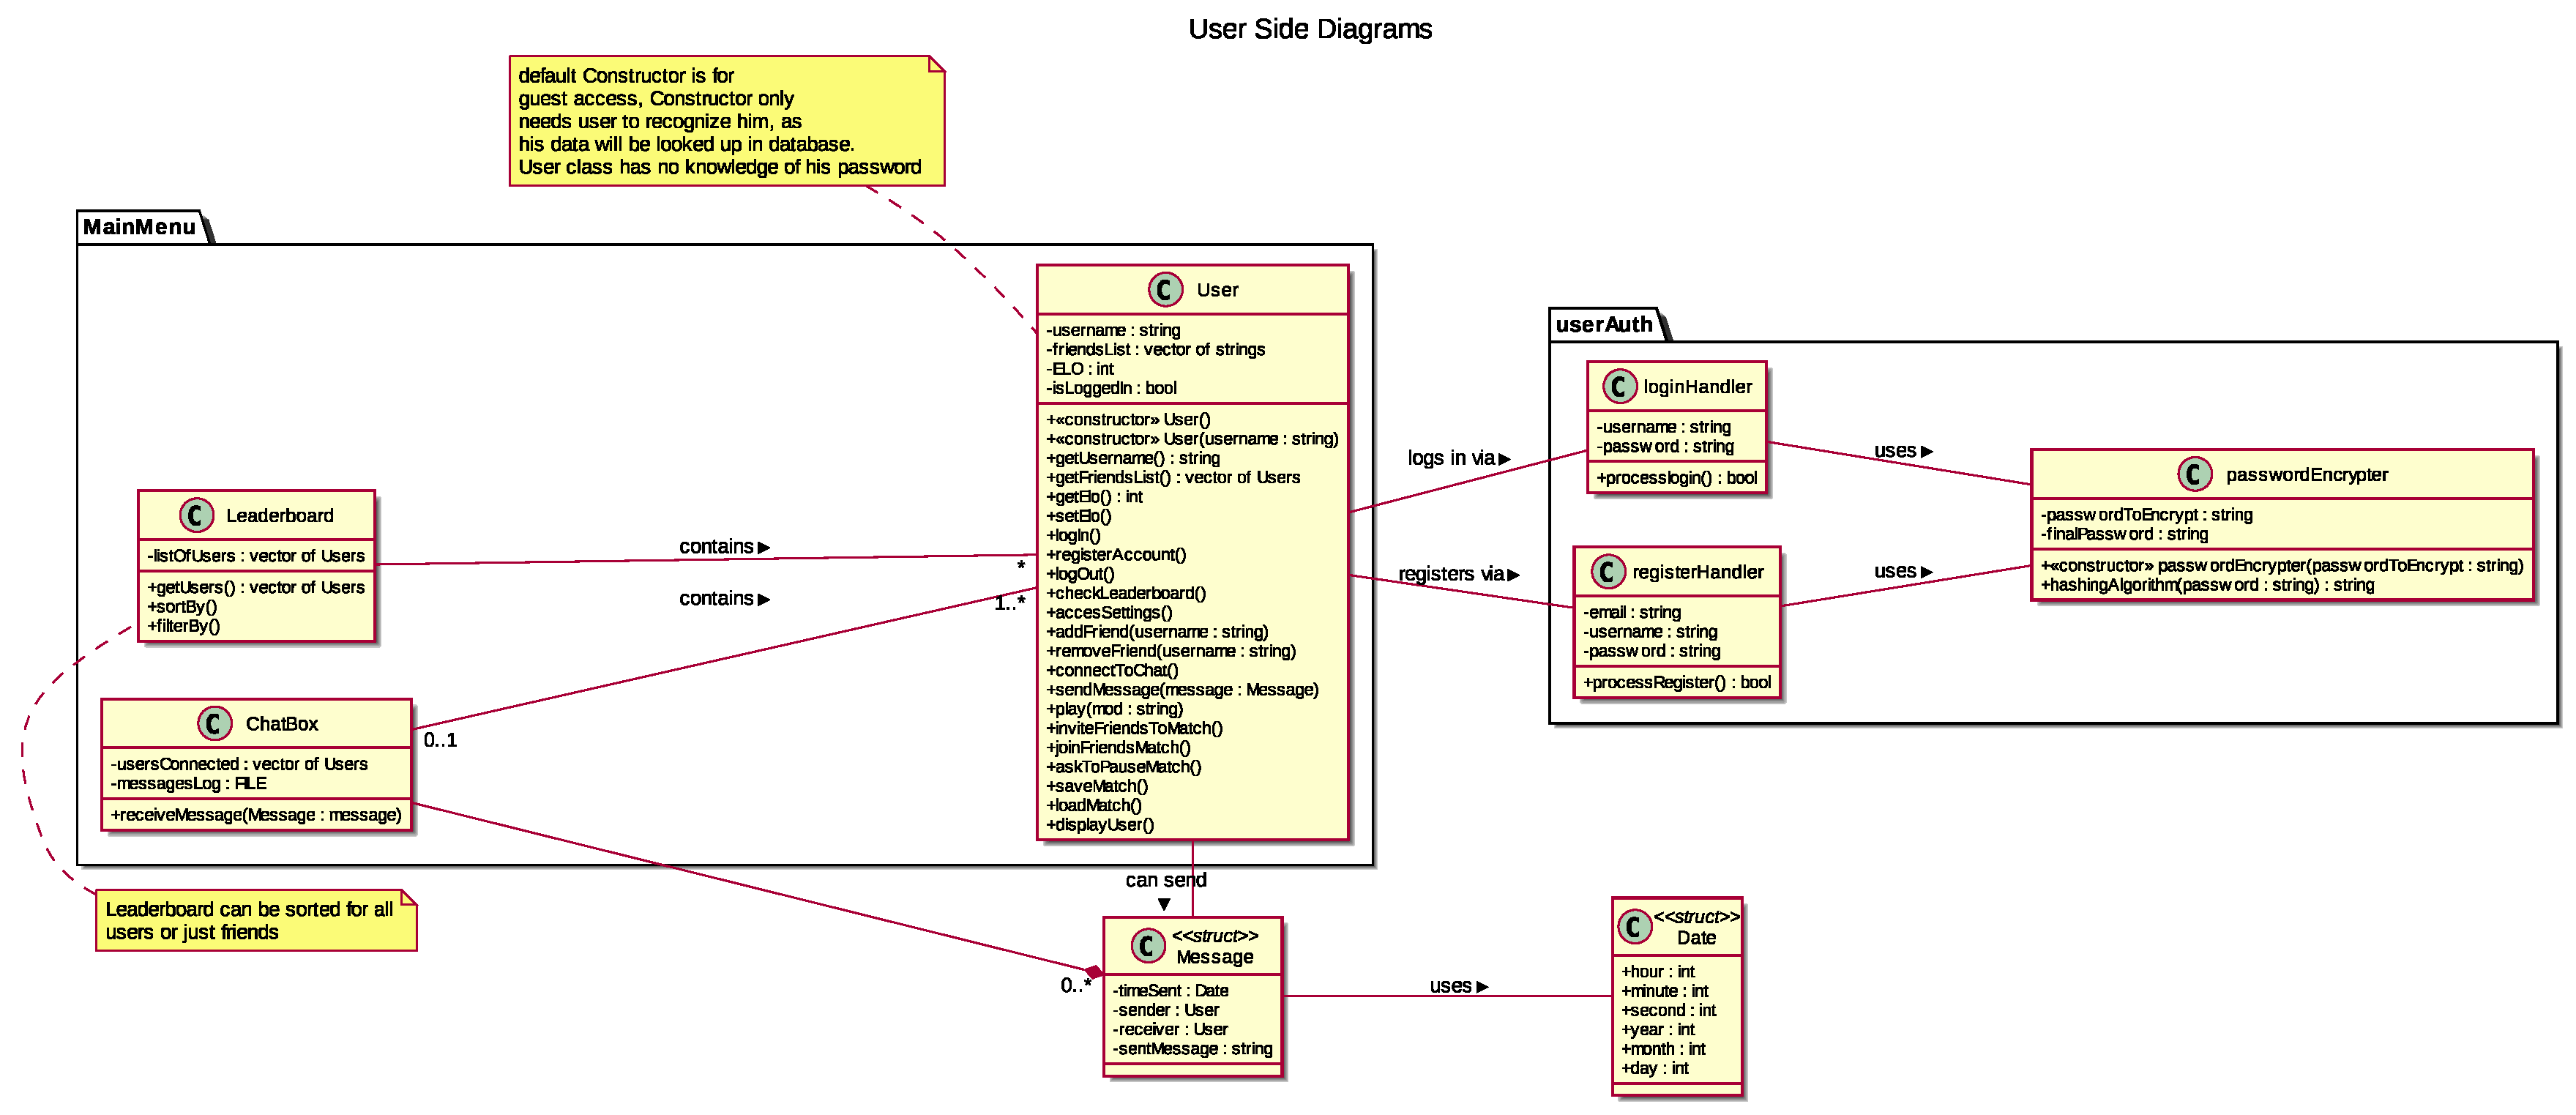
\includegraphics[width=\textwidth]{UserSideDiagrams.eps}}
    \addimg{img/6_UserSideDiagrams.eps}{width=\textwidth}{Diagrammes du côté utilisateur}{usrside}
        L'utilisateur entre dans le jeu comme une sorte de "Guest",
        ne pouvant pas utiliser l'interface
        Pour pouvoir utiliser les fonctionnalités de Quoridor, l'utilisateur doit se connecter
        à son compte ou en créer un s'il n'en a pas. Les deux evenements passeront à travers des "handlers", qui
        géreront les requetes en passant à travers un database et le Server. Après s'etre connecté.e, l'utilisateur aura accès à toutes les fonctionnalités
        que offre le logiciel (cfr. Sections 2 et 4).
    \subsubsection{Coté jeu}
        % \makebox[\textwidth]{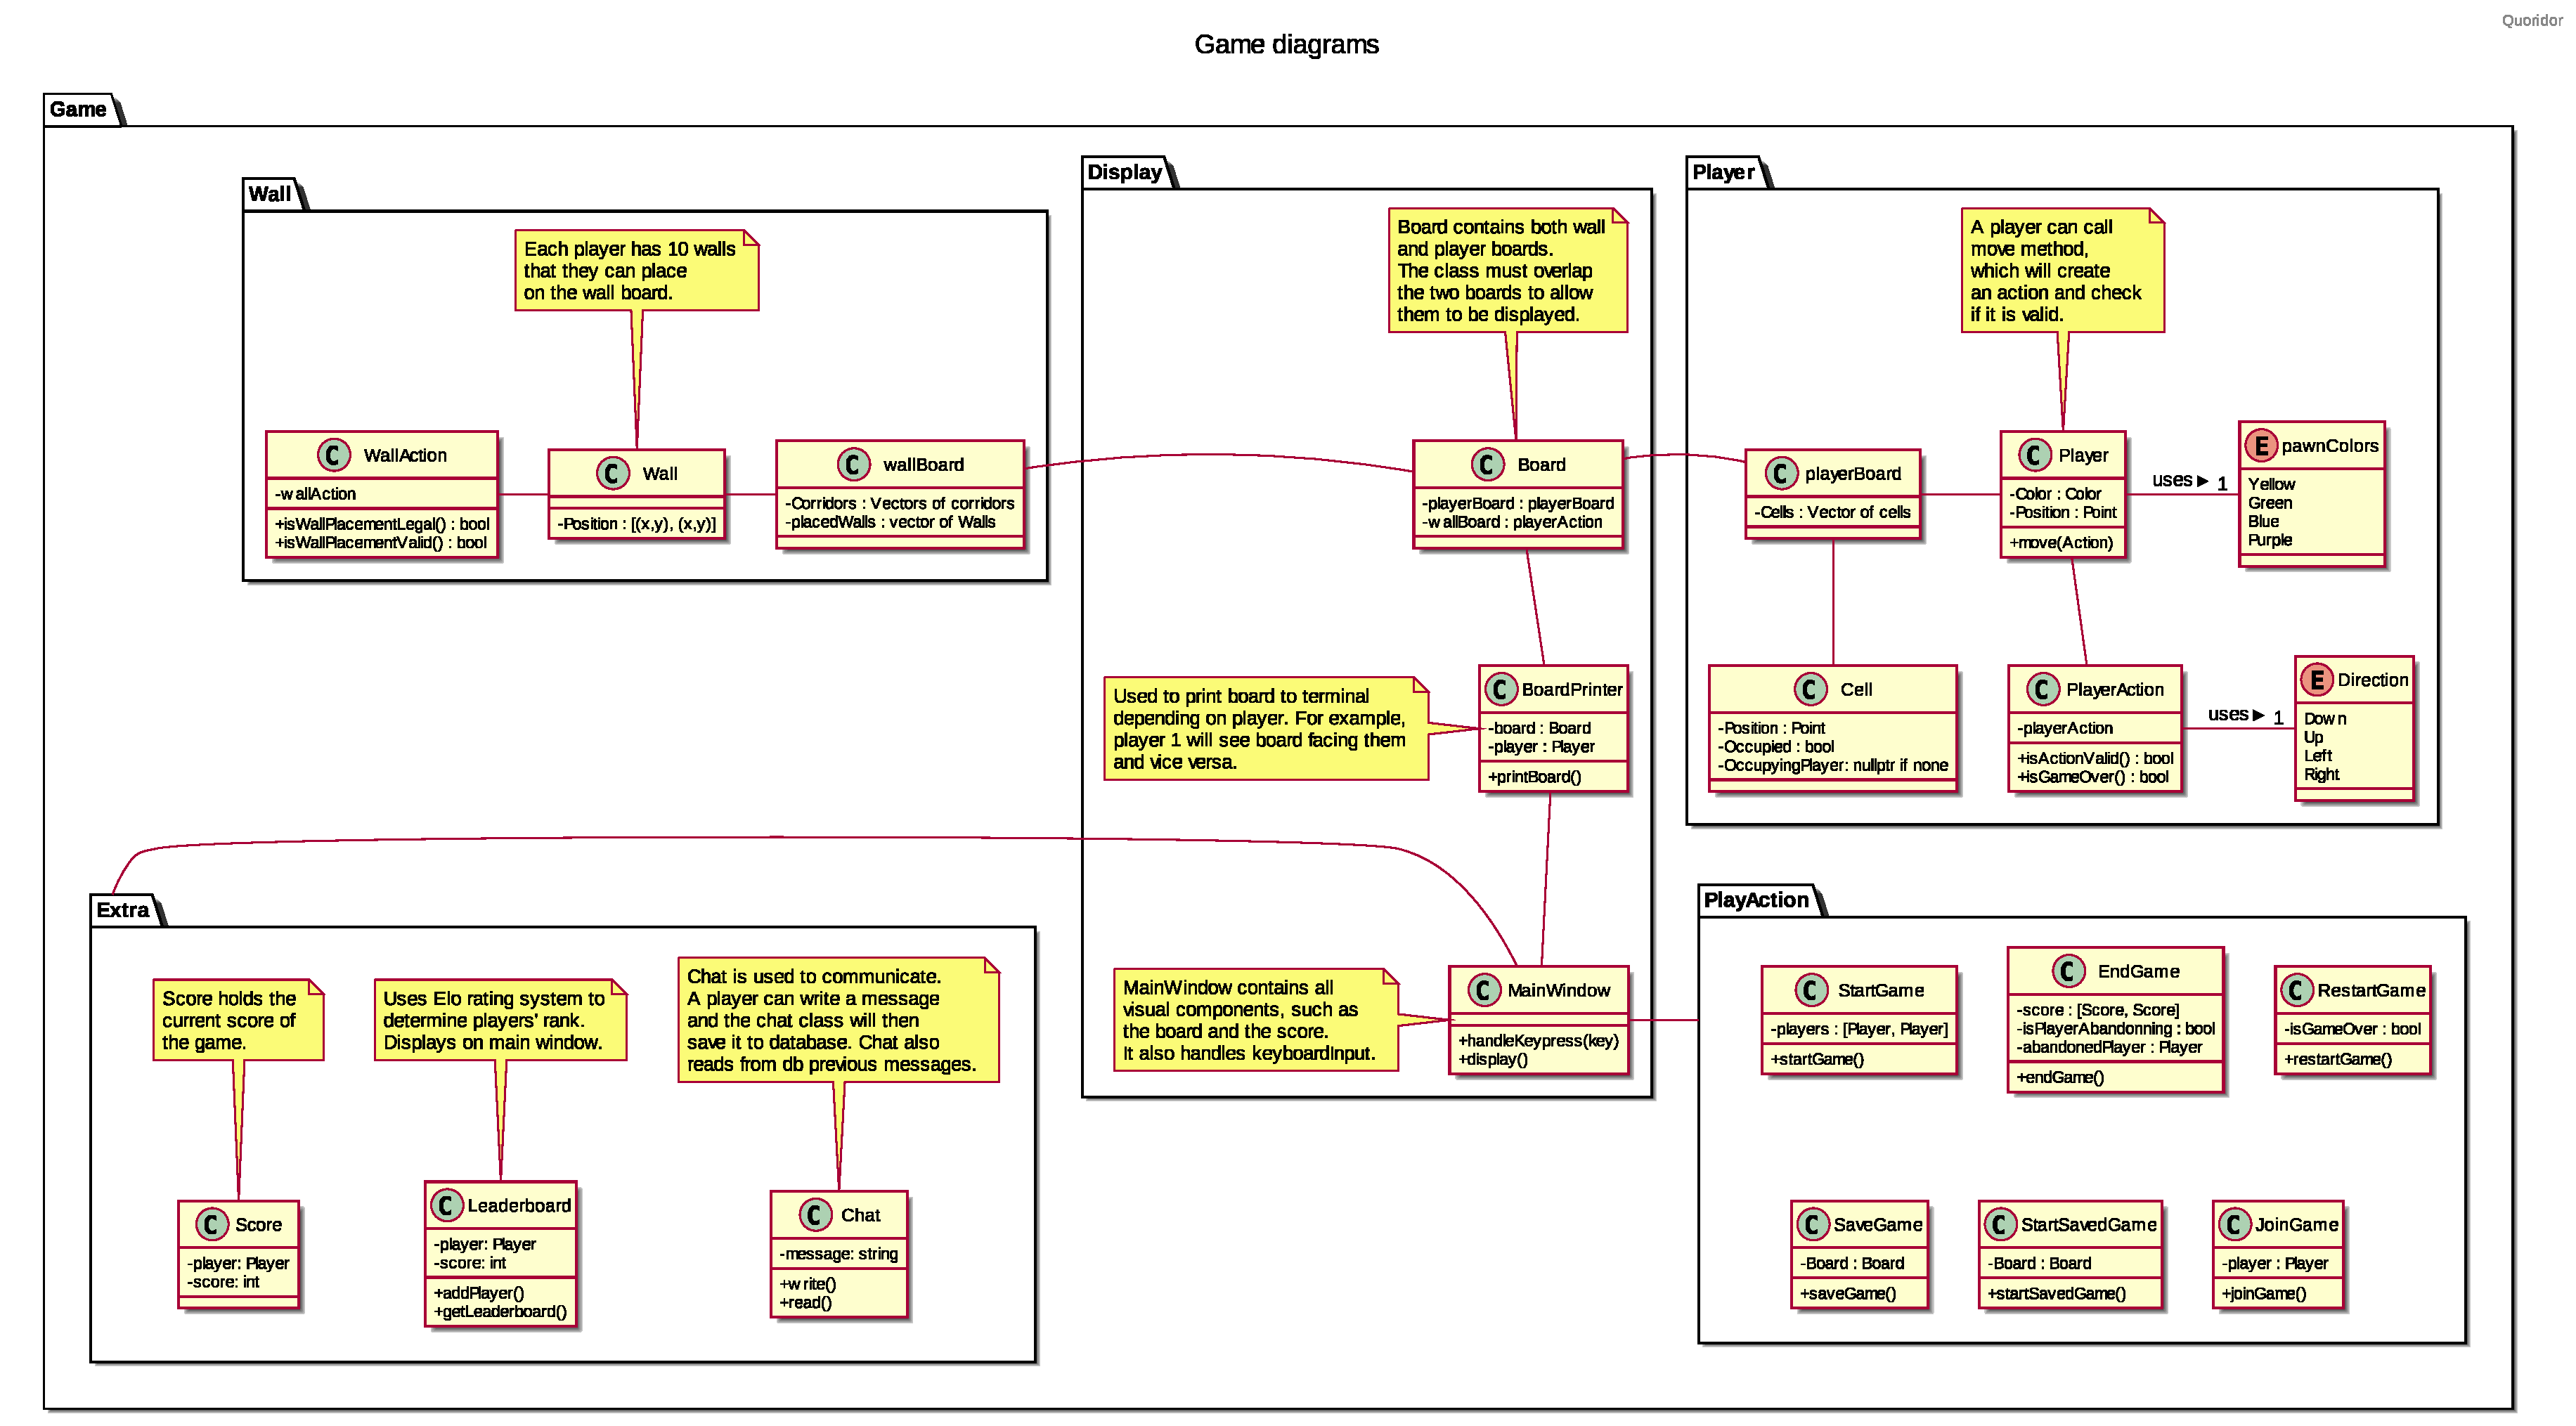
\includegraphics[width=\textwidth]{GameDiagrams.eps}} 
    \addimg{img/6_GameDiagrams.eps}{width=\textwidth}{Diagrammes de jeu}{gameside}
        Le jeu est divisé en deux plateaux. Le plateau mur (Wall board) contient les murs. Alors que le plateau joueur contient les pions des joueurs. Chaque pion a une couleur différente afin de permettre aux joueurs de se différencier l'un de l'autre. La classe board combine chaque plateau, qui sera ensuite afficher par BoardPrinter dans MainWindow. 
        
        Le PlayerBoard est divisé en cases. Chaque case peut accueillir au maximum un pion définit par la classe Player. Chaque Player peut se déplacer sur le PlayerBoard en faisant appel à la classe PlayerAction, qui vérifie si le coup est valide.
        
        Le WallBoard est quant à lui est divisé en couloir. Chaque couloir peut contenir un Wall. Un couloir a une largeur de 2 cells.
        L'utilisateur peut placer un wall en faisant appel à WallAction qui va d'abord vérifier si l'action est valide.
    

